\documentclass[12pt]{scrartcl} %for better layouts
\usepackage{setspace}
\usepackage{graphicx}
\usepackage{amsmath}
\usepackage{natbib} %for citet and citep
\usepackage{syntonly}
\usepackage{esdiff} %for writing partial derivatives
\usepackage{url} %for inserting urls

%\syntaxonly for quickly checking document

%set document settings
\doublespacing % from package setspace

\title{The Effect of Oil Price on Field Production}
\subtitle{Evidence from the Norwegian Continental Shelf}
\author{
  		Johannes Mauritzen \\
        Department of Business and Management Science\\
        NHH Norwegian School of Economics\\
        Bergen, Norway \\	           
		}
\date{\today}

\begin{document}
\begin{spacing}{1} %sets spacing to single for title page
	\maketitle
\end{spacing}

\begin{abstract}
An increase in oil prices could affect oil production in a particular region in three ways.  Higher oil prices could lead to increased exploration, starting production in known but previously uneconomic fields or to changes in production in existing fields.  While several studies exist on the effect of oil prices on exploration, to my knowledge no studies exist of the effect of oil price on production in existing fields.  I use detailed data on Norwegian oil field production and a semi-parametric additive model to control for the production profile of fields.  I find no significant evidence of a concurrent reaction of field production to oil prices, though a slight lagged effect is found of the magnitude of approximately 2 to 4\% for a 10 dollar per barrel increase in the real price of oil.  These findings are consistent with the idea of producers that do not act strategically to short-term price movements but instead use storage and financial derivatives to hedge oil price changes.  
\end{abstract}


\section{Introduction}

For most of the last century, crude oil has been the world’s single most important and valuable fuel source.  Naturally, questions of how the oil price affects the world economy as well as how oil production reacts to the oil price have been fundamental topics in economics. However a significant gap exists in the literature.  While numerous studies have taken up the issue of how oil prices affects searching for new fields as well as total oil production at both the regional and global level, to my knowledge no studies exist of the effects of oil prices on oil production at the field level.  

The effect of oil prices on production from existing fields is an important topic, both as an empirical counterpart to the extensive theoretical literature on optimal extraction and more generally in understanding the mechanisms of how total oil supply reacts in response to price.  The response of oil production in existing fields is especially important now as many of the major oil-producing areas, like the Norwegian continental shelf are mature and an increasing amount of oil production comes from existing fields rather than new finds.  How production from these fields will respond to lower or higher oil prices has major implications for both the state finances of oil-producing countries such as Norway as well as for total world oil supply and long-run oil prices.  

%Implications for theories and explanations for understanding of the price mechanism and %the role of speculation.  Hamilton block quote.  

The lack of research on the role of price in oil field production is likely due to two main factors - the availability of data and the non-linear time profile of field production.  Large private oil companies, notably the “super majors” and state-owned oil companies have historically accounted for the vast majority of oil production and reserves. \footnote{See for example the economist article titled Supermajordämmerung from August 3rd, 2013: \url{http://www.economist.com/news/briefing/21582522-day-huge-integrated-international-oil-company-drawing}} These entities tend to consider field-level data as either company or state secrets.   

Luckily a notable exception to the general rule of inaccessible data exists.  The Norwegian government has committed itself to transparency in the petroleum sector and detailed data on most aspects of the country’s oil industry is openly available.  I use historical production data from all 77 currently or formerly oil-producing fields on the Norwegian continental shelf in order to estimate the effect that prices have on oil production.  

By looking only at the effect of price on fields that currently or previously have produced oil I am limiting the scope of this article.  The effect of oil prices on total production over an extended period of time is due not just to reactions in production in existing fields but also increased searching for new fields.  In fact, an implication of this work is that much of the total production response from higher oil prices is from increased searching as well as production from previously un-economic fields.

The main finding in this article is that oil production at the field level has no significant reaction to concurrent changes in the oil price, where concurrent is broadly defined as within the first three years.  A slight effect can be detected at a lag of between 4 and 6 years, with a magnitude of about a 2 to 4\% increase in yearly production for a 10 dollar increase in the price of oil.  This effect is somewhat greater and with less of a lag in large fields compared to small fields.

The main methodological problem, as mentioned, is the non-linear production profile of oil fields.  Once full scale extraction is started in an oil field, pressure in wells will quickly drop.  Technological solutions such as gas and water injection also have quickly declining effectiveness.  In turn production will drop quickly. 

More so, oil field production is correlated across fields - that is, increases and decreases in production in fields are not randomly distributed across time.  Instead, as figure \ref{top10_production} shows with the production profile of the 10 largest Norwegian oil fields, production tends to be correlated across fields.  The result is a total production curve that is bell shaped over time as in figure \ref{oil_decline}.  Since oil prices are autocorrelated, a failure to properly account for the production profile will lead to spurious estimation of the price terms in a regression.  

The direction of this bias can be gleaned in figure \ref{oil_decline}.  High oil prices were present at periods of relatively low production in the late 1970s and early 1980´s as well as over the last 10 years, however real prices reached some of their lowest levels at the same time as the top of production around the year 2000.  This inverse relationship is entirely accidental, but will heavily bias the estimation of the effect of price on production if the production profile at the level of the oil field is not properly accounted for.  

\begin{figure}
	\includegraphics[width=.8\textwidth]{top10_production.png}
	\caption{}
	\label{top10_production}	
	\end{figure}

\begin{figure}
	\includegraphics[width=.8\textwidth]{oil_decline.png}
	\caption{}
	\label{oil_decline}
\end{figure}

As a solution I use a semi-parametric model within the Generalized Additive Model frameworks of \cite{hastie_generalized_1990}.  Here I use a two-dimensional smoothed spline function to account for the general non-parametric shape of the production profile while allowing price to enter the equation linearly.  The coefficient of price can then be interpreted as the average effect of price on production over the entire production profile.

\section{The effect of oil price on production: theory and empirics}
The question of the effect of oil prices on production and the more general question of optimal oil extraction has a long history and goes back to the seminal work of \citet{hotelling_economics_1931}.  The theoretical literature on optimal extraction is too vast to cover even at a superficial level, however \citet{krautkraemer_nonrenewable_1998} provides a good overview.  At a basic level however, a central idea of much of this theoretical work is that with a non-renewable resource, production is a decision that involves a significant opportunity cost: more production in the current period means less production in future periods.  Within this frameworks, prices and expectations of prices become important variables in the production decision.  

For modeling aggregate oil production, shape-fitting models, notably \citet{hubbert_energy_1962} and more recently advocated by \citet{deffeyes_hubberts_2001}, have had some success in estimating the timing of peak production at the regional and national level, but they tend to seriously underestimate the total recoverable resource of oil-producing regions and the models can be shown to be fundamentally misspecified \citep{boyce_prediction_2013}.   Simulation type studies where aggregate oil production is modeled through a often complex combination of physical and economic processes also exist in the geo-engineering literature, but their usefulness tends to be weighed down by their complexity as they require quite detailed data and specific assumptions about functional form that can be difficult to justify \citet{brandt_review_2010}.

More important to this paper are empirical estimates of the effect of price on production. Several econometric papers seek to answer the question of how aggregated oil supply is affected by oil prices.  \citet{farzin_impact_2001} attempts to estimate an elasticity for the effect on added reserves of increased oil prices and finds a small though statistically significant effect.  \citet{ramcharran_oil_2002} estimates a supply function for the total supply of oil from several OPEC countries based on data from 1973 to 1997.  The author finds a negative price elasticity for several of the countries, and interprets this as evidence of producers targeting revenue.  However since the author does not take into account the production profile of oil fields and the spurious correlation that can arise with autocorrelated prices, these estimates come under considerable doubt.  

the effect of oil-price uncertainty on drilling and exploration has also been explored.  \citet{kellogg_effect_2010} finds that oil exploration firms in Texas do approximately respond as real-option theory would predict when it comes to the timing of drilling.  A model and test using data from North Sea producers on the UK continental shelf by \citet{hurn_geology_1994}, on the other hand, fails to find evidence that the variance in the oil price affects the timing of oil field development.  I do not attempt to directly model uncertainty, however given that the investments needed to increase oil production in an existing field are to a certain extent irreversible and that oil prices are highly volatile, the results can and probably should be interpreted with the real options framework in mind.  

One of the few studies to use field level data is \citet{black_is_1998} that tests the relevance of “nesting” a structural empirical model of profit maximization that takes into account oil prices into a typical geo-engineering model of oil field production.  They find strong evidence that taking into account profit maximization, and implicitly price, substantially improves the fit compared to a purely geo-engineering type model.   The limitation of their methodology is that they are only able to test whether including economic factors like price affects the fit of the model but are not able to give an estimate of the effect.  Methodologically, the paper also relies heavily on assumptions about the functional form of both the geo-engineering aspects of the oil producer as well as their profit-maximization.  By taking a more flexible, semi-parametric approach to estimating the effects of oil field production profile, this paper avoids problems with overly restrictive assumptions.  

Studies using detailed Norwegian data on offshore activity also exist, though the focus has mainly been on exploration and drilling.  \citet{mohn_exploration_2008} finds that long-term changes in the oil-price has a strong effect on exploratory drilling though little effect is measured from short-term changes in the oil price.  \citet{osmundsen_exploration_2010} analyses drilling productivity over time on the Norwegian Continental Shelf while \citet{mohn_efforts_2008} finds that higher oil prices leads to higher reserves by way of both greater efficiency in searching as well as greater effort.  

\section{Oil production on the Norwegian Continental Shelf}
The first commercial oil well in Norwegian continental waters was discovered in December of 1969 in what became the Ekofisk oil field, the largest Norwegian oil field by estimated recoverable reserves.  As figure \ref{north_sea_reserves} shows, most of the largest fields in the North Sea were found relatively early on while more recent finds have tended to be smaller - a pattern typical of oil producing areas called creaming.  A major exception to this trend was the recent find of the Johan Sverdrup field which is estimated to have approximately 300 million SM3 of recoverable oil. \footnote{The Johan Sverdrup field is estimated to begin producing oil in 2017 and so is not present in the data set used for the analysis.}  

\begin{figure}
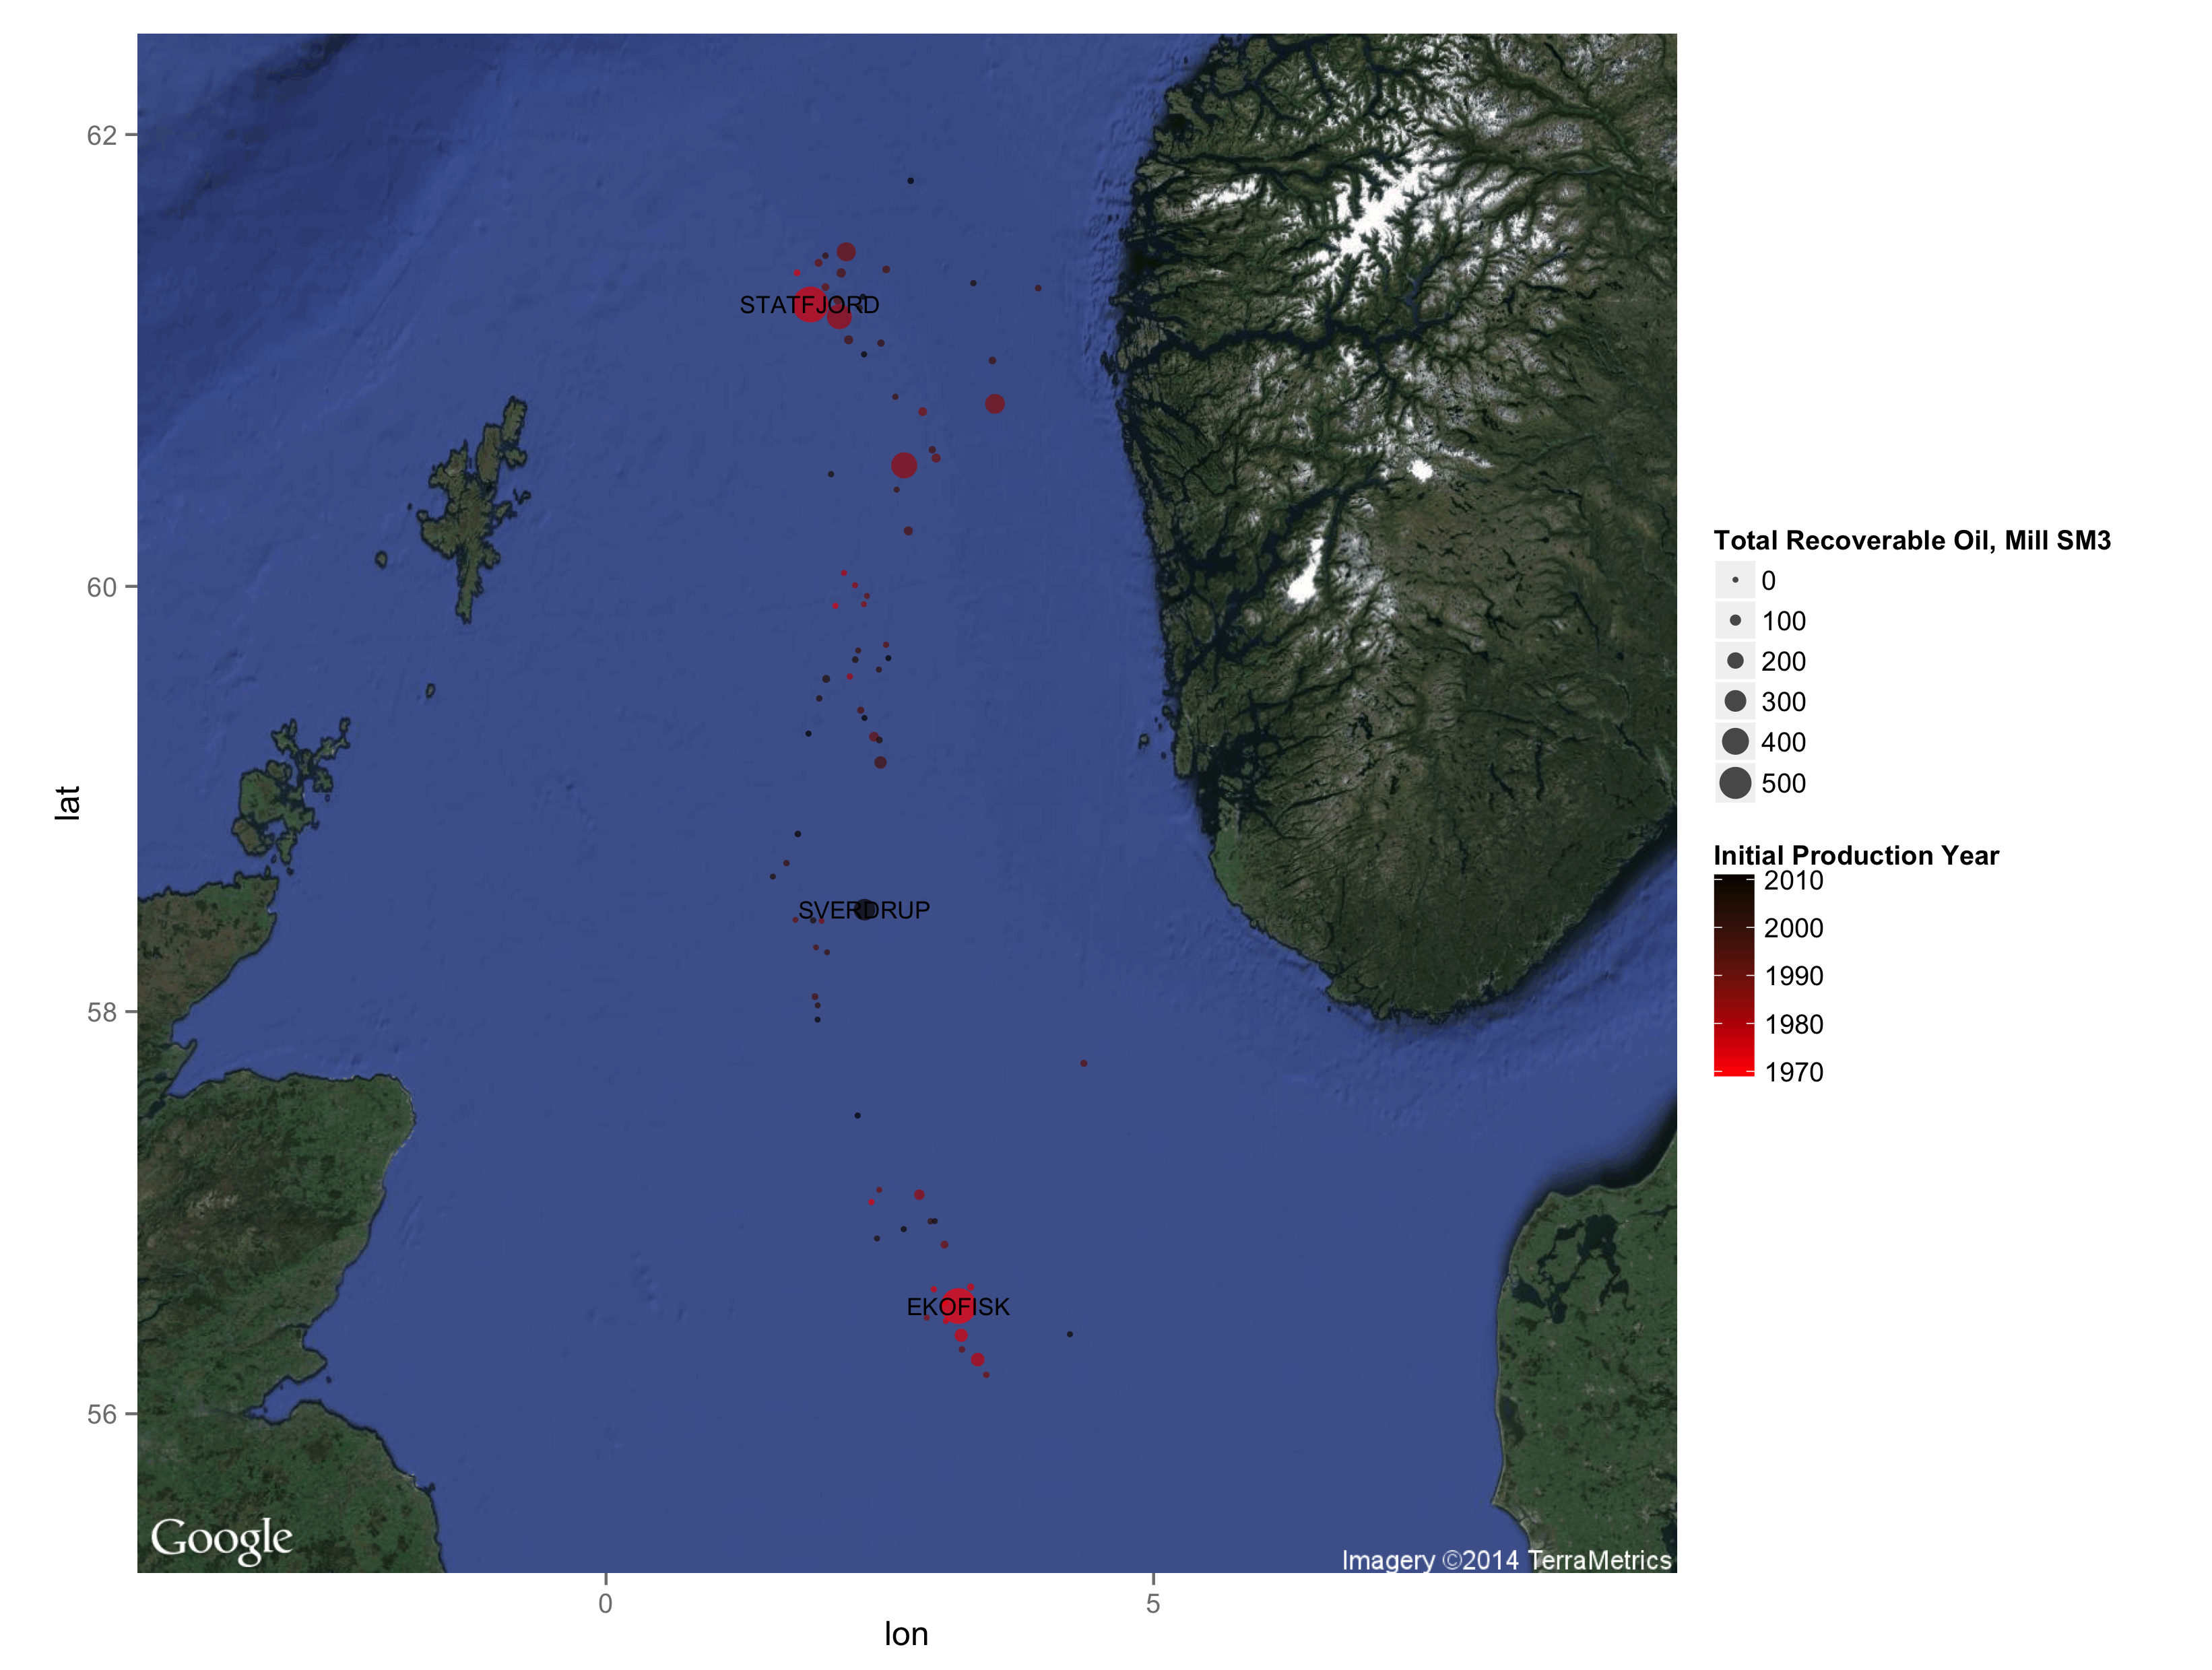
\includegraphics[width=.8\textwidth]{north_sea_reserves.png}
\caption{}
\label{north_sea_reserves}
\end{figure}

Exploration in the Norwegian sea was opened in the early 1980’s and the first commercial field started production in 1981.  While several mid-sized fields have been discovered, the Norwegian Sea has generally disappointed in terms of commercial oil finds and most finds have been relatively small (\ref{norwegian_sea_reserves}).  

\begin{figure}
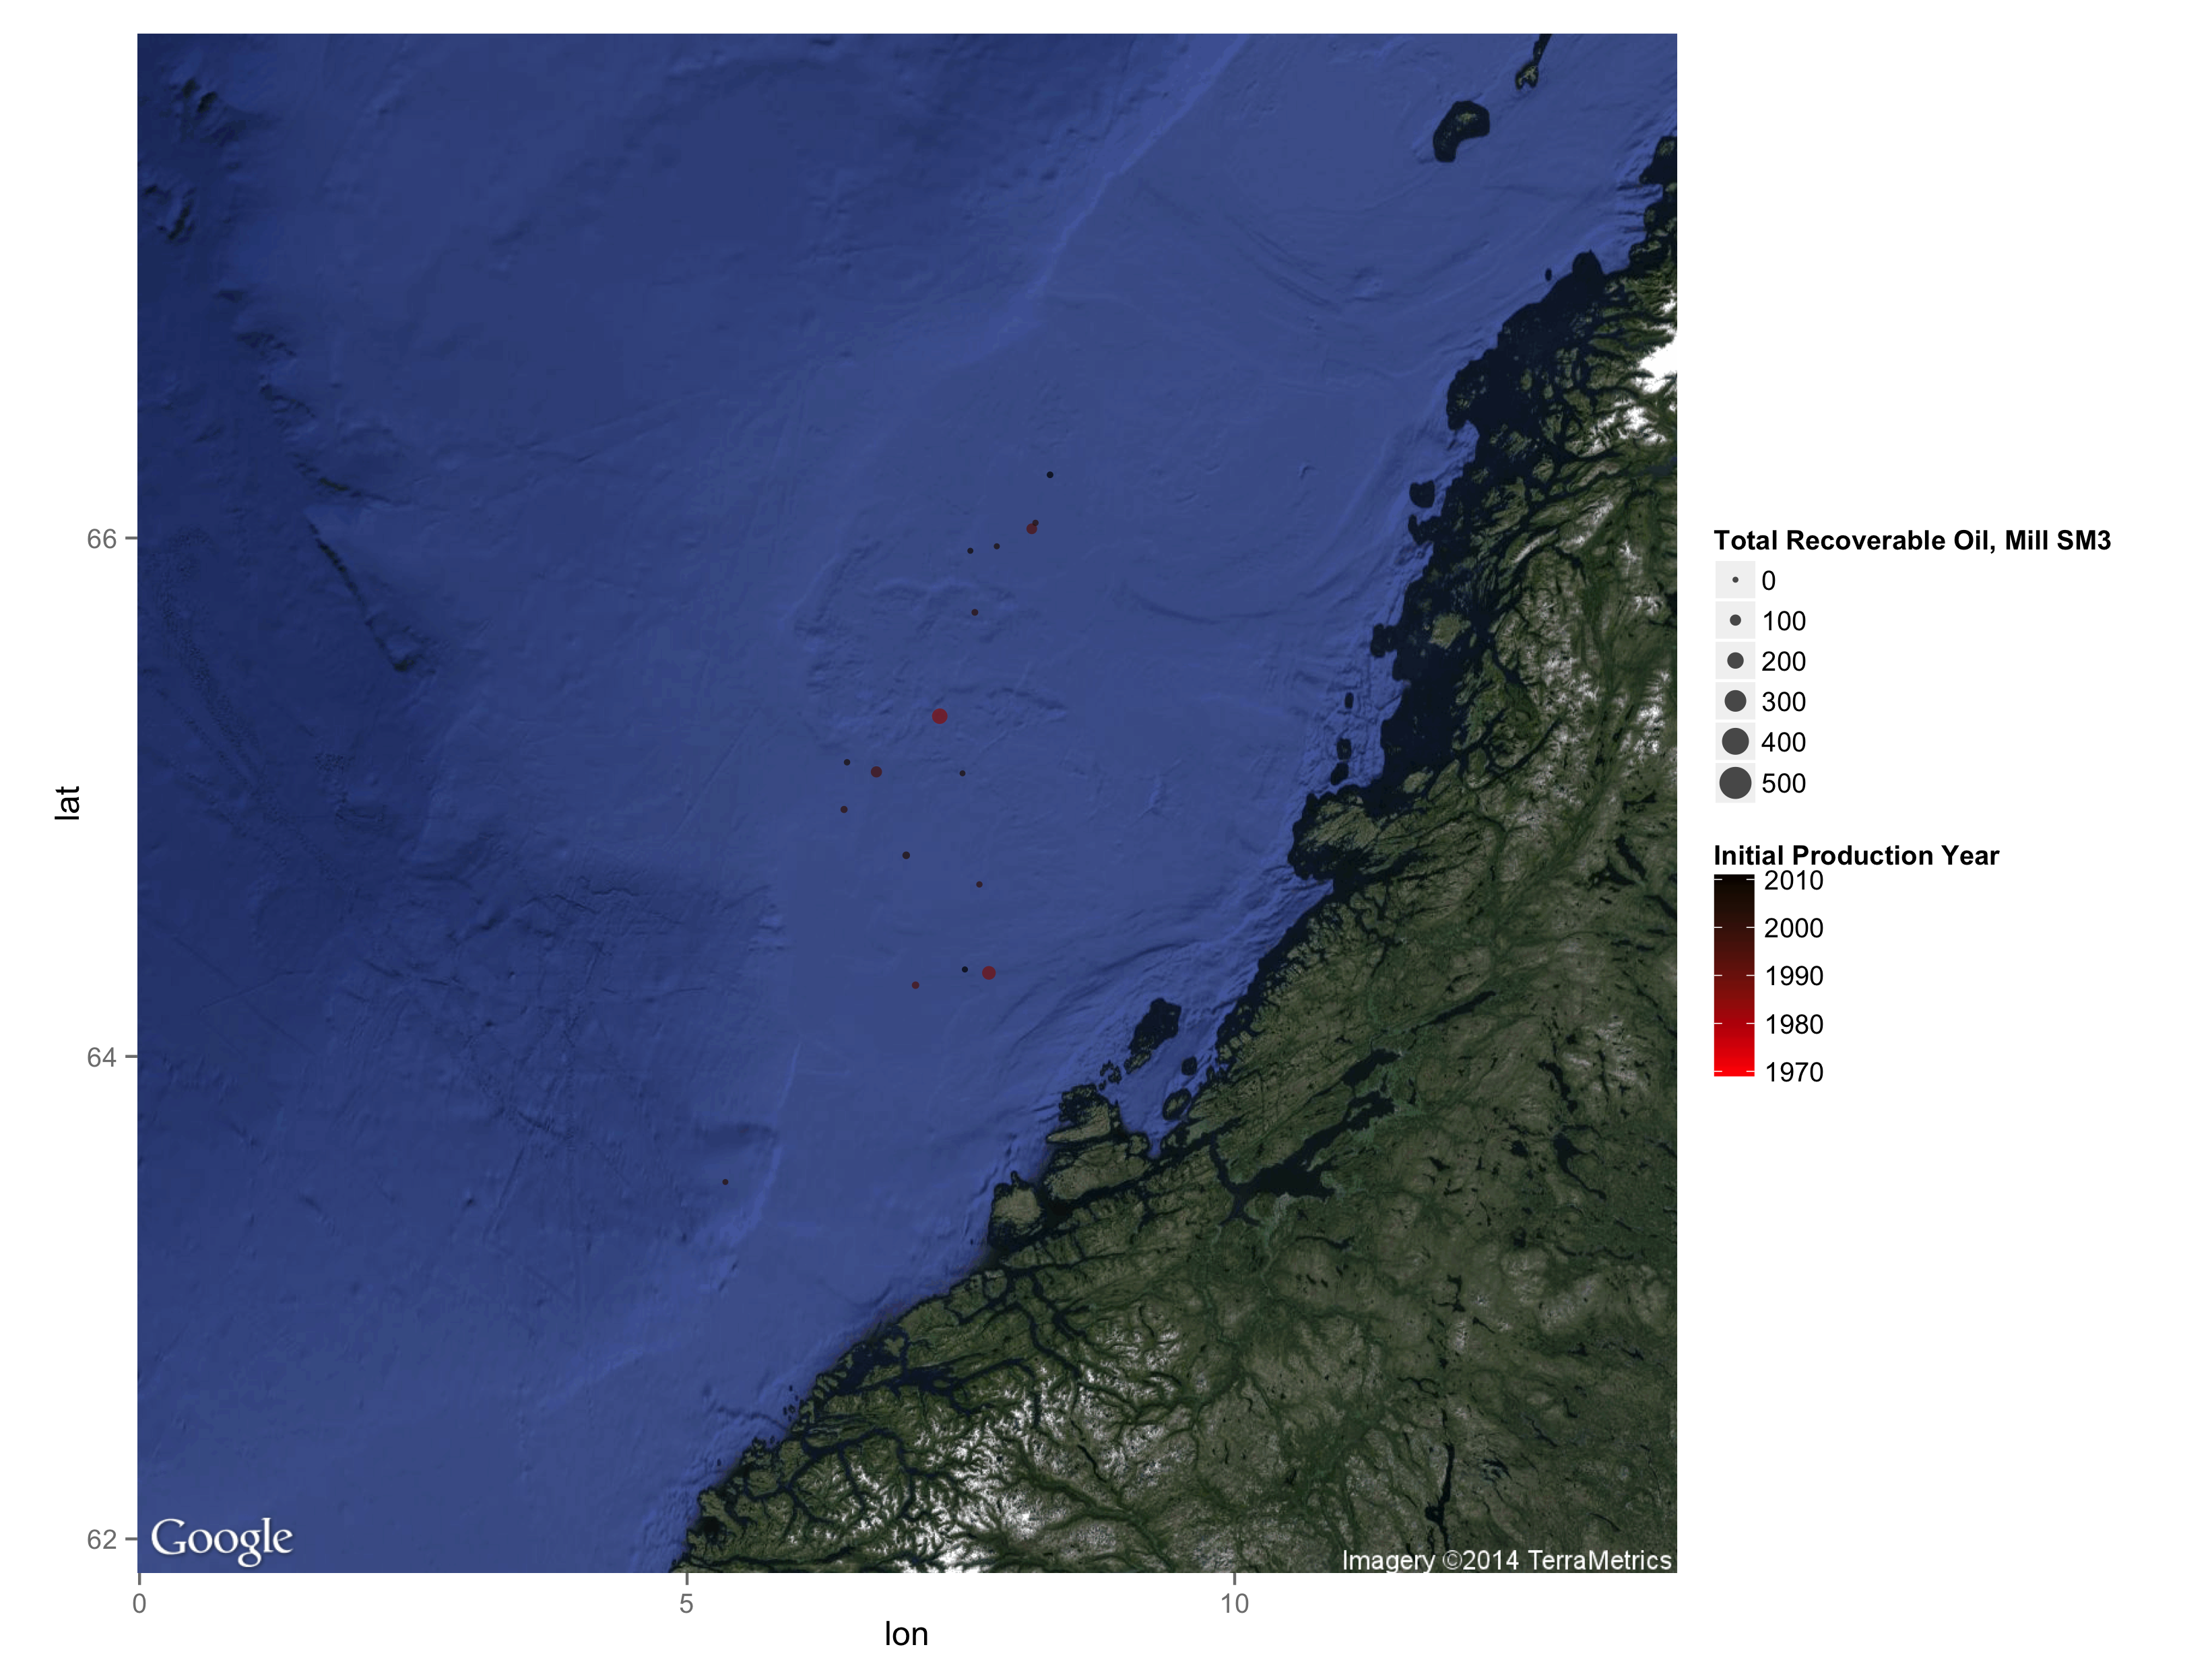
\includegraphics[width=.8\textwidth]{norwegian_sea_reserves.png}
\caption{}
\label{norwegian_sea_reserves}
\end{figure}

Norwegian waters in the Barents sea have also been open to exploration since the 1980s, however up until recently only a few, small finds were made and none came into commercial production.  However recently several significant oil and gas finds have been made in the Barents Sea - notably the oil field Goliat and the large gas find Sn\o hvit, which are both currently under development but not yet producing.  The agreement between Norway and Russia in June 2011 settling a long-running dispute over the maritime delimitation has also given a boost to new exploration in the region.  

Profits from oil and gas production in Norway are subject to a resource tax of 50 percent on top of the ordinary income tax of 28 percent, thus income from petroleum production is taxed at a total marginal tax rate of 78 percent.  The central government also receives revenues through ownership stakes in companies, notably Statoil, where the state is the majority stakeholder.  This over-all tax rate has been fairly constant through the history of Norwegian oil production, however several important changes related to the tax code have occurred.  In 1991 a C02 tax was introduced, but this was mainly levied on the use and import of petroleum products.  In the offshore sector it was levied on the burning of oil and gas and thus the main effect was on the practice of flaring natural gas that could not be transported and sold commercially.   

More importantly to the offshore sector were accounting changes that were implemented in 2002 and 2005 that were meant to encourage new entrants by allowing losses to be carried forward for tax purposes and by introducing a rebate on the tax-value of losses associated with searching and drilling.  In general though, these rules mainly affected searching and discoveries of new fields rather than production from existing fields and I do not control for the tax changes in my model.  More information on taxation and revenues from the offshore sector can be found at the website of the Norwegian Ministry of Finance. \footnote{\url{http://www.regjeringen.no/en/dep/fin/Selected-topics/taxes-and-duties/bedriftsbeskatning/Taxation-of-petroleum-activities.html?id=417318}}

Rights to explore and eventually produce on the Norwegian Continental Shelf are based on a system where the government announces geographic blocks that will be opened to oil exploration and production subject to production licenses.  Production licenses are initially granted for between 4-6 years subject to requirements that firms are actively searching in their awarded blocks.  If oil or gas deposits are proven then the production license can be extended for up to 30 years.  In general, the frameworks are fair, predictable and stable for companies who find commercially extractable oil deposits and regulatory interference is unlikely to be the cause of any observed changes in production from existing oil fields.  For more information see the website of the Norwegian Petroleum Directorate. \footnote{\url{http://www.npd.no/en/Topics/Production-licences/Theme-articles/Production-licence--licence-to-explore-discover-and-produce-/}}

\section{Norwegian oil field production data}
Production data of Norwegian oil fields is obtained from the website of the Norwegian Petroleum Directorate \footnote{http://factpages.npd.no/}  Production data is available at a monthly frequency for all fields, though I choose to aggregate up to yearly values both to smooth over seasonality as well as short-term volatility of output due to factors such as weather or technical issues.  

In addition to data on field-level production, I also make use of data on estimated total recoverable reserves.  The use of this variable is complicated as it is an estimate subject to a large amount of uncertainty, especially in relatively young fields.  However, the methodologies used to estimate the total recoverable resource of a field are constantly evolving and it is a fair assumption that any consistent bias of the estimates are observed in older fields and corrected for in estimates for newer fields.  I can then assume that existing errors are random and will not overly bias the estimates.  

I use yearly data from the US Energy Information Agency on the real price of Brent-traded oil in 2010 dollars.  The Brent benchmark oil price is likely the best oil price measure for Norwegian production as it is based on light sweet crude oil sourced from the North Sea.  

An argument can be made that expectations of future oil prices can be equally if not even more important for production decisions as the current oil price.  Forecasts for future oil prices are available from, among others, the International Energy Agency, but these have tended to be notoriously inaccurate and it is unlikely oil companies use these projections for their investment decisions.  On the other hand, given the size and liquidity of oil spot markets, it is a fair assumption that the current oil prices do a good job of incorporating much of the available information about crude oil markets and that future price movements are generally difficult to predict \citet{hamilton_understanding_2008}.  An active futures market does exist, but several studies have found that current oil prices are in general better than prices on futures contracts at predicting future oil prices \citep{alquist_what_2010, chinn_predictive_2005}.

A cleaned data set and the full code for the analysis can be found at my website \url{jmaurit.github.io# oil_prices}. I use the R statistical programming package for all the analysis in this article \citet{team_r:_2013}.  In addition I use the R packages ggplot2 and ggmap for plotting \citep{wickham_ggplot2:_2009, kahle_ggmap:_2013}, plyr for data manipulation and cleaning \citep{wickham_split-apply-combine_2011}, and mgcv for implementation of the Generalized Additive Models \citep{wood_fast_2011}.

\section{A generalized additive model of oil field production}
Parametric linear models have the sizeable advantages of simplicity and interpretability and therefore usually a good starting point for an analysis.  However, when attempting to model the effect of price on oil field production, a standard linear model is unable to sufficiently control for the production profile and therefore heavily biases the estimate of the effect of price.  As an example, consider a generalized linear model written as in equation \ref{glm_eqn}. 

	\begin{equation}
	\begin{split}
	 Log(Production_{i,t}) & = \alpha_0 + \alpha_1 time\_to\_peak_{i,t} + \alpha_2 time\_to\_peak_{i,t}^2 \\
	& \quad + \alpha_3 time\_to\_peak_{i,t}^3  + \alpha_4 peak\_to\_end_{i,t} + \alpha_5 peak\_to\_end_{i,t}^2 \\
	& \quad + \alpha_6 peak\_to\_end_{i,t}^3 + \gamma total\_recoverable\_oil_i \\
	& \quad + \beta_1 oil\_price + \beta_2 oil\_price\_l1 + ...+ \epsilon
	\end{split}
\label{glm_eqn}
	\end{equation}

Here the left hand side variable is yearly production in year $t$ for field $i$.  To try to account for the time profile of production, I split up model time into a time-to-peak and peak-to-end variable as demonstrated for data for the Statfjord filed in figure \ref{statfjord_dem} and then represent each as a cubic function.  Yearly production is assumed to be proportional to the total size of the field as represented by the estimate of the total recoverable resource.  Finally, a term for the oil price as well as 5 lagged terms are added in order to capture the effects of price.  

\begin{figure}
\includegraphics[width=.8\textwidth]{statfjord_dem.png}
\caption{}
\label{statfjord_dem}
\end{figure}

Figure \ref{glm_dirty_box} shows the estimates of the coefficients on the oil price and its lags \footnote{The dots on the figure represent 1000 simulations of the estimated coefficient based on the estimated standard error and point estimate from the model}.  The lags are not estimated to have an effect significantly different from zero. However a literal interpretation of the coefficient on the concurrent oil price term would indicate that a 10-dollar increase in the oil price would lead to a lowering of field production of around 2\%.

\begin{figure}
\includegraphics[width=.8\textwidth]{glm_dirty_box.png}
\caption{}
\label{glm_dirty_box}
\end{figure}

This estimate is of course heavily biased downwards due to the spurious correlation between the field production profiles and the autocorrelated time series of oil prices.  The parametric representation is not flexible enough to control for the production profile of the fields.  Instead, a more flexible estimation of the production profile is needed. 

Instead of attempting to estimate the shape of the production profiles of the fields by estimating parameters on linear terms I estimate a non-parametric function for the production profile.  As an illustration, consider the production profile of a single field.  The simplest possible model would then have the form of equation \ref{simp_eqn}. 

\begin{equation}
Production_{t}=f(time) + \epsilon
	\label{simp_eqn}
\end{equation}

Again considering the production profile for the Statfjord field, a smoothed function might look like the black line in figure \ref{statfjord_gam}.   

\begin{figure}
	\includegraphics[width=.8\textwidth]{statfjord_gam.png}
	\caption{}
	\label{statfjord_gam}
\end{figure}

In principle any number of well-behaved smoothers could be used to estimate the function, for example a Loess or a kernel smoother.  In practice regression splines are most commonly used.  With a regression spline the data points for the function to be estimated are broken into bins.  For each bin of data a local linear regression is estimated.  For functions of one variable, a cubic parameterization is often used.  These regressions are then essentially tied together at what are called “knots” and the smoothness of the overall function is controlled by a penalty function that consists of the second derivative of estimated function.

In my regression, I find it helpful to represent the production profile of fields as a two-dimensional function.  This can not be accomplished with a standard cubic regression spline, but I can instead use a Thin Plate (Regression) Spline \citet{wood_thin_2003}.  Though the full details of the implementation are well beyond the scope of this paper, for the basic idea consider equation \ref{thin_plate_1}.  

	\begin{equation}
	y_i = g(x_1, x_2)
	\label{thin_plate_1}
	\end{equation}

Following \citet{wood_generalized_2006}, $g$ is the function of $x_1$ and $x_2$ that is to be estimated by $f$, which in turn is estimated by minimizing \ref{thin_plate_2}.  Here $boldsymbol{y}$ represents a vector of $y_i$’s and $boldsymbol{f} = (f(boldsymbol{x_1}),f(boldsymbol{x_2}))^t$.   

	\begin{equation}
\min \|\boldsymbol{y-f}\|^2 + \lambda J_{22}(f)
\label{thin_plate_2}
	\end{equation}

$J_{22}$ represents the penalty function for the smoothness of the function which can be written as in \ref{thin_plate_3}.  The $22$ represents the fact that it is a penalty function of two variables with smoothness measured by the second derivative.

	\begin{equation}
	J_{22}{f}= \diffp[2]{f}{x_1}^2 + \diffp[2]{f}{{x_1}{x_2}} + \diffp[2]{f}{x_2}^2dx_1 dx_2
\label{thin_plate_3}
	\end{equation}

In short, a function of $x_1$ and $x_2$ is found that is minimizing errors in the sense of minimizing euclidian distance subject to a penalty function of “wiggiliness”.  The actual implementation is somewhat more involved in order to increase the computational efficiency of the estimation.  For further details I again refer to \citet{wood_thin_2003}.

The advantage to using splines over other smoothing methods is that it can be represented in a linear form.  Thus estimation of the model can be done using standard and efficient matrix algebra algorithms. For further details I refer to the discussion in \citet{hastie_generalized_1990} and \citet{wood_generalized_2006}.  The latter is a particularly useful reference for implementing generalized additive models in R.  As a general note, this paper is not meant as a methodological piece.  The methods used here, while still not common in economics, are mature, developed and commonly used in statistics as well as by other empirical researchers.

Of course, I do not want to estimate smoothed curves individually for each field.  While this would provide a good overall fit to the full data set, it would not be particularly informative.  Instead I want to estimate a general shape of the production profile for all fields and then use the remaining variation in the data to see what effect price has.  My model can be written as in equations \ref{gam_price_eqn}.

\begin{equation}
\begin{split}
	Log(Production_{i,t})&=f(time\_to\_peak_{i,t}, total\_recoverable\_oil_i) \\
	& \quad + f(peak\_to\_end_{i,t}, total\_recoverable\_oil_i) \\
	& \quad + \beta_1 oil\_price + \beta_2 oil\_price\_l1 + ... +  \epsilon
\end{split}
\label{gam_price_eqn}
\end{equation}

In this model I am estimating the parameters and functions from all fields $i$. As in the parametric model presented earlier, the left-hand-side variable is yearly oil production for field $i$. Also like the parametric model I split the production-time component element in two: up to and after the peak in production.  While a shape for the entire production profile could be estimated with one smoothed function, splitting it up allows for more flexibility and better overall fit of the model as estimated by deviance score and the related estimated degrees of freedom of the model.  

I also allow the smoothed functions to vary with the total size of the field as measured by the estimated total recoverable oil since the shape of the production profile tends to vary substantially by field size.  Inspection of a selection of fields, such as shown in figure \ref{field_inspection}, shows that smaller fields tend to reach their peak quickly while larger fields, which need to be built up in order to reach their full production, take more time.

\begin{figure}
	\includegraphics[width=.8\textwidth]{field_inspection.png}
	\caption{}
	\label{field_inspection}
\end{figure}

Even with a smoothed function that is allowed to vary by field-size, a substantially better fit could be obtained by splitting the estimation into small and large fields, this time measured by max production year.  The improvement in fit can be seen by inspecting the fitted values of the models as in figure \ref{bench_vs_split}. The split estimation provides a particularly better fit for smaller and mid-sized fields.

\begin{figure}
	\includegraphics[width=.8\textwidth]{bench_vs_split.png}
	\caption{}
	\label{bench_vs_split}
\end{figure}

\section{The Effect of Oil Price on Field Production}

The variables of interest is of the course the oil price and its lags, which I include as seven linear parametric terms in the model.  The idea of including both a concurrent oil price term as well as six lags is that a change in price could conceivably have two effects on oil production in a field.  First, the field operator could be operating on the basis of some short-term extraction rule - choosing to pump out less at times of lower prices so that they could pump out more at periods of high prices.  

Alternatively, a change of oil prices can be seen as a lifting of a production constraint.  A higher oil price means that is worthwhile to invest more in production in order to either increase the total amount extracted from a field or to shift production forward.  However investments in the offshore sector can be complex and thus are implemented with a considerable lag.  

The estimates of the parametric oil price terms are shown in figure \ref{gam_price_dirty_box}.  What is shown is a box plot centered around the point estimate of each coefficient.  The box can be interpreted as a 50 percent confidence interval while the lines can be interpreted as a 95% confidence interval.  Estimates for fields with a maximum yearly production of over and under 8 million SM3 are shown.  

\begin{figure}
	\includegraphics[width=.8\textwidth]{gam_price_dirty_box.png}
	\caption{}
	\label{gam_price_dirty_box}
\end{figure}

The estimated coefficients for the concurrent and first three lags of the oil price are not estimated to be significantly different than zero.  For large fields a modest effect at the fourth and sixth lags are estimated while for small fields an effect is estimated only at the sixth lags. The magnitude of these effects is in the neighborhood of a 2\% increase in production for a 10 dollar increase in the oil price.  

As can also be seen from the figure, these estimates are right on the margin of the traditional 95 percent confidence threshold.  However the estimates do make some intuitive sense.  Discussions with people in the industry about the results also supports their validness.  In general, operating an oil production rig and related infrastructure is an extremely expensive venture with high fixed costs.  In the challenging conditions of the North Sea, the expenses are multiplied.  Thus any short term benefit of strategically altering production in relation to movements in the oil price are dominated by the large costs of having excess capacity.  In other words, oil producers have a strong incentive to pump as much oil out at any given time given the existing production capacity.  

Instead, the results point to a mechanism where oil producers react to higher oil prices by increasing investment in those fields, which comes on-line and leads to higher oil production only with a considerable lag.   This story is in line with a trend of increased total extraction estimates from the Norwegian continental shelf as a whole as well as from existing fields over the last 15 years of strongly rising oil prices \footnote{\url{http://npd.no/Templates/OD/Article.aspx?id=4731&epslanguage=en}}.

Another potential motive is that higher oil prices leads companies to expand the production rate in the face of uncertain future oil prices.  While not strategic in the sense discussed earlier of having spare capacity ready and reacting to short-term price movements, it would mean companies are changing their level of investment in order to shift the production profile over time - a higher price induces companies to produce more relatively sooner thus leaving less in the ground for future production.  In reality, the motive is likely a combination of the above factors - an oil price induces investment in increased production capacity in order to both shift forward production as well as increase the overall extraction rate.  

In the above discussion, I have been implicitly giving the coefficients a causal interpretation, which deserves some discussion.  My main identifying assumption is that production on the field level can not cause significant changes in the oil price.  A stronger but still relevant assumption that may be necessary since field production is correlated across fields is that total production from the Norwegian continental shelf does not affect oil price.  Both of these assumptions are likely satisfied.  Oil is a globally traded commodity and total Norwegian production accounts only for a small fraction of total production.  In 2013 Norwegian production made up only 2.3 percent of the world total \footnote{\url{http://www.eia.gov/countries/country-data.cfm?fips=NO#pet}}.  A drastic change in production, on par with the halt in production that occurred in Libya in 2011 \footnote{Before the Libyan revolution of 2011, Norwegian and Libyan yearly oil production were of a similar magnitude, 2.1 versus 1.8 million barrels of oil in 2010, \url{http://www.eia.gov/countries/country-data.cfm?fips=LY#pet}}, would have been required to have had any significant effect on world oil supply and in turn prices. 

One of the main implications of the interpretation that higher oil prices leads to increased extraction through increased capacity is that while the effect on production will be lagged, higher oil prices will have a more immediate effect on investments.  I test for this with the model as written in equation \ref{gam_invest_eqn}

\begin{equation}
\begin{split}
	Log(Investment_{i,t})&=f(time\_to\_peak_{i,t}, total\_recoverable\_oil_i) \\
	& \quad + f(peak\_to\_end_{i,t}, total\_recoverable\_oil_i) \\
& \quad + \alpha oil_production_{i,t} \\
	& \quad + \beta_1 oil\_price + \beta_2 oil\_price\_l1 + ... +  \epsilon
\end{split}
\label{gam_invest_eqn}
\end{equation}

In the equation investment in each field $i$ at time $t$ is a function of the state of field development, as modeled by a non-parametric function of time to and from the peak as well as the total size of the field - as in the model of oil field production.  In addition I include a term for oil production in field $i$ at time $t$.  The coefficients of interest are again those on the oil price and its lags.  

The results for the estimation of the estimated coefficients on the oil price and its lags is shown in figure \ref{gam_price_invest_box}.  The coefficient on the concurrent oil price as well as the first two lags are all significantly positive, with coefficients that can be interpreted to mean that a 10 dollar increase in the oil price leads to between a 5 to 10 percent increase in oil field investment for the current and two subsequent years.  No significant effect can be estimated for subsequent lags however

\begin{figure}
	\includegraphics[width=.8\textwidth]{gam_price_invest_box.png}
	\caption{}
	\label{gam_price_invest_box}
\end{figure}

The results of the regression on investment fits nicely with the previous results on oil production which showed a significant effect in the 4th through 6th lags.  A story consistent with both results is that higher oil prices induce increased investment in production capacity, though it takes time to get the extra capacity in place and the effects on production to be felt.

\section{Conclusion}

\begin{figure}
	\includegraphics[width=.8\textwidth]{field_lev_forecast.png}
	\caption{}
	\label{field_lev_forecast}
\end{figure}

\begin{figure}
	\includegraphics[width=.8\textwidth]{tot_forecast.png}
	\caption{}
	\label{tot_forecast}
\end{figure}

\begin{figure}
	\includegraphics[width=.8\textwidth]{price_scenario.png}
	\caption{}
	\label{price_scenario}
\end{figure}

The results of this paper are important in themselves in helping explain and decompose the effects of price on oil production.  Production in existing fields has no significant concurrent reaction to higher oil prices while a slight effect is estimated  with a lag of between 4 and 6 years.  Oil producers do not appear to be behaving strategically in relation to short-term production - increasing or reducing production in response to changes in oil price.  Instead they are likely using storage or financial instruments to hedge short-term price movements. Changes in oil prices can rather be seen as a relaxing of a production constraint, justifying increased investment that leads to either a higher total extraction rate or a intertemporal shifting of production. 

The modest estimated effect of prices on production adds evidence to the argument of \citet{hamilton_oil_2012} that most of the increased supply of oil that comes from higher prices is from expanding the geographic and technological boundaries of oil production.  For example exploration of deep-water oil deposits off the coast of Brazil and extraction of oil sands in western Canada.  

Beyond the explanatory importance of the results, the Generalized Additive Model methodology, which to my knowledge has not been used in either geo-engineering nor econometric studies of oil production, can also serve a useful function in producing forecasts and scenarios.  The major advantage that the methodology has is that by estimating an overall function for the production profile of fields, then production from newer fields can be estimated based on the history of older fields.  In this way, forecasts of total oil supply from a region can be built in a bottom-up and relatively simple way that avoids overly restrictive assumptions. 

While a full forecasting model is outside the scope of this paper, I illustrate the potential with a simple forecast.  An important caveat here is that I am forecasting total oil production from existing fields.  Production from new fields are not estimated.  Figure \ref{field_lev_forecast} shows the forecast at the field level for several of the fields while figure \ref{tot_forecast} shows the aggregated forecast.  The different scenarios are for oil prices that increase or decrease by a fixed amount per year in order to reach a certain oil price in the year 2022 as shown in figure \ref{price_scenario} .  

Visually, the forecasts appears sensible.  As would be expected from the results, the different oil price scenarios only lead to different outcomes after a several year delay.  An equally important point is how even a large difference in oil price leads to relatively minor change in expected production.  

Overall, the forecast is likely to be somewhat downward biased.  The reason is that in the model, forecasts of future production from newer fields are based on the production path of older fields.  However, technological change is likely to improve the overall production rate of newer fields.  However, if history is any indication, the effect of technological change on production from existing areas will be modest \citep{hamilton_oil_2012}.

The forecasting results of this model are presented in this article for illustrative purposes and a good deal more work would need to be done, especially in estimating an appropriate measure of uncertainty for the forecasts.  Nonetheless, the results of the model provide a striking contrast to the much more optimistic projections of oil production from the Norwegian Petroleum Directorate even when accounting for projected production from existing fields. \footnote{\url{http://www.npd.no/Templates/OD/Article.aspx?id=4648&epslanguage=en}}


\bibliographystyle{plainnat}
\bibliography{oil_prices}

\end{document}
This is never printed